\section{Introduction}
% problem description: semantic relatedness
Computing semantic relatedness(SR) between two elements(words, sentences,
texts etc.) is a fundamental task for many applications in Natural Language
Processing(NLP) such as lexicon induction\cite{aaai/QadirMGL15}, Named 
Entity Disambiguation\cite{acl/HanZ10}, Keyword Extraction
\cite{ijcai/ZhangFW13} and Information Retrieval\cite{acl/GurevychMZ07}. 
Besides those NLP applications, in the aspect of opinion spam problem\cite{www/SandulescuE15}
and image classification\cite{iwcs/LeongM11}, semantic relatedness measurement plays a great role as well. 
In this paper we focus on computing semantic relatedness between two words based on entity comparison in knowledge graph.

It has long been thought that when humans measure the relatedness between a pair of words,
a deeper reasoning which requires a large amount of knowledge is triggered to compare the concepts behind the words.
In the past years, many researchers have worked for semantic relatedness measurement and have made great achievements.
From the aspect of data resources which they used, there are:
i) \emph{The lexical databases} such as WordNet\cite{acl/Pucher07} or Wikithionary\cite{aaai/ZeschMG08} play a great part in
relatedness measurement. This data resource provides precise lexical information, but misses the semantic information.
ii) WikiRelated\cite{aaai/StrubeP06}, ESA\cite{ijcai/GabrilovichM07}, WLM\cite{aaai/ZeschMG08} and so on exploit \emph{the large corpora wikipedia}
to compute semantic relatedness. Wikipedia-based methods usually outperform the lexical-based methods, 
because the wikipedia which is built artificially contains abundant semantic information. 
iii) Recently, there are some researchers having attached importance to measure semantic relatedness
in knowledge graph. 
The SensEmbed \cite{acl/IacobacciPN15} leveraged BabelNet\footnote{http://babelnet.org} to annotate the dump of wikipedia,
and exploited word2vec\cite{corr/Mikolov13} to train the sense-annotated wikipedia to get distributed representation of different 
word senses. Essentially this method is based on \emph{the large corpora} and needs a significant preprocessing
and data transformation efforts. 
The REWOrD \cite{aaai/Pirro12} is purely knowledge graph based model which proposed an approach which exploited 
the graph nature of RDF and SPARQL query language to access knowledge graph. It not only obtained the comparable
result with the state-of-art model at that moment, but also avoided the burden of preprocessing and data transformation.
% Another model BabelRelated!\cite{aaai/NavigliP12} proposed a knowledge-rich approach to compute multilingual semantic
% relatedness which exploited the joint contribution of different languages. 

\begin{figure*}
    \flushleft
    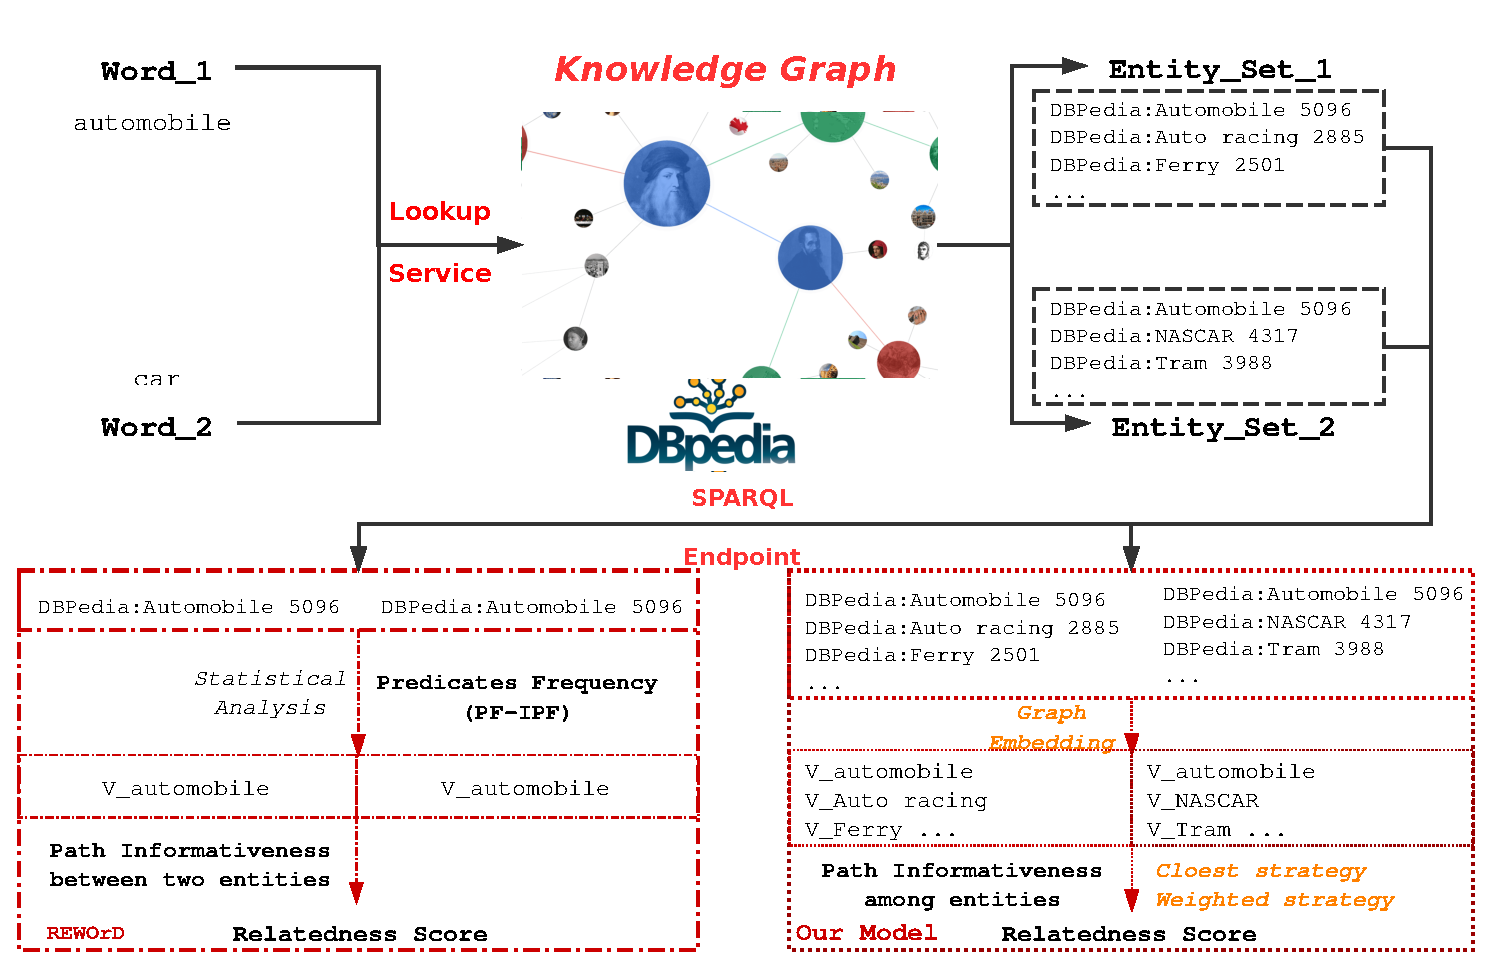
\includegraphics[width=1.0\textwidth]{pic/overview.eps}\\
    \caption{Subgraph in knowledge graph}
    \label{overview}
\end{figure*}

Though REWOrD\cite{aaai/Pirro12} achieved great balance between
semantic relatedness measurement and data preprocessing.
However, they missed some factors which might contribute to semantic relatedness measurement. 
Firstly given two words as input, the first step is to find corresponding entities in knowledge graph.
Obviously, there are usually more than one corresponding entities for a single word.
As show in figure \ref{overview}, for an input word \emph{automobile}, for example, 
we will get \emph{DBPedia:\footnote{http://dbpedia.org/resource}Automobile} and
\emph{DBPedia:Auto\underline{\hspace{0.5em}}Racing}, \emph{DBPdedia:Ferry} and so on.
From the lower-left corner of figure \ref{overview}, we can see that the REWOrD lost sight of
the informativeness of the other entities, while they just consider the entity with the highest rank.
Secondly, REWOrD missed some informativeness of \emph{objects} in \emph{triple(subject, predicate, object)}
because their strategy just took the \emph{predicates} into account with statistics of frequencies based on the TFIDF exclusively.
This method ignored the information hidden in \emph{objects} in a semantic triple.

%阐述我们的model%
To get an approximation to human relatedness judgement more accurately and exploit more knowledge implied in knowledge graph,
we propose an improved model based on entity comparison in knowledge graph. 
As show in figure \ref{overview}, given two words in input, the first step is to get entities that better associated with 
the concepts triggered by input words. To this end we rely on lookup services provided by DBPdedia which is used in REWOrD as well. 
In contrast to REWOrD, we consider multiple entities associated with input words rather than just one with hightest rank.
Along with the idea which transforms the entities to vector which can be compared easily, we need to get the vectorization representation
of entities. However, traditional statistical analysis methods used in REWOrD can not consider both knowledge hidden in \emph{predicates}
and \emph{objects} in semantic triple. To make up this weakness, we use graph embedding to train the dataset which contains subgraphs
extracted from knowledge graph. Due to the huge amounts of data in knowledge graph, it is difficult to extract the minimal subgraph which
can describe the entities accurately. We do this by building a directed graph which contains all relevant entities and attributes which
describe the entities set. After training and computing the distance between vectors, we can get multiple relatedness scores.
We use two \emph{weighted} strategy to combine the relatedness scores as the final semantic relatedness score. Experimental
results show that our model outperforms the REWOrD and some of other wikipedia-based methods.

In this paper, we propose a threefold model.

i) Given a pair of words, the first job is to query the corresponding entities. In order to use the
embedding technique to train the dataset, we construct a graph which contains all related
entities, attributes and relations between the corresponding entity pairs.

ii) We exploit embedding technique for knowledge graph instead of Word2vec to train the subgraph
extracted from the knowledge graph. Then we can get a distributional representation(vector) for each
entity and predicate.

iii) We can get multiple relatedness scores after a full link between these two sets of entities.
Inspired by \cite{acl/IacobacciPN15}, we utilize an approach to combine the relatedness scores as the final semantic relatedness score.

This paper is organized as follows. We give the related work about semantic relatedness
measurement in section \ref{related-word}. Then we elaborate the threefold model for
computing relatedness scores in section \ref{methodology}. Finally, we display detailed
illustrations of experiment results which show that our model outperform the state-of-the-art model.

% In the past few years, With the development of knowledge representation, utilizing knowledge-rich resources to compute semantic 
% relatedness is a well-explored line of research because knowledge graph contains richer syntactic and semantic information
% than lexical databases, and more structured knowledge than the large corpora.

% Knowledge graph can be accessed with powerful query language Sparql in RDF graph.
% As for the methods build on the data soruce, the recent word embedding 
% learning approaches demonstrate their abilities
% to capture syntactic and semantic information, and outperform the
% lexicon-based methods\cite{acl/Pucher07}. 
% Knowledge Graph, as a semantic graph, stores
% vast amount of structured knowledge. 

% Recently, there are some researchers having attached importance to measure semantic relatedness
% in knowledge graph\cite{acl/IacobacciPN15}, \cite{aaai/NavigliP12}, \cite{aaai/Pirro12}. 
% The SensEmbed \cite{acl/IacobacciPN15} leveraged entity linking to annotate the dump of wikipedia,
% Then word2vec\cite{corr/Mikolov13} is used to train the sense-annotated wikipedia and they got distributed representation of different 
% word senses. Essentially this method is based on \emph{the large corpora} and needs a significant preprocessing
% and data transformation efforts. The knowledge graph plays a role of support network in SensEmbed.
% Another model BAbelRelated!\cite{aaai/NavigliP12} proposed a knowledge-rich approach to compute multilingual semantic
% relatedness which exploited the joint contribution of different languages. 
% The REWOrD \cite{aaai/Pirro12} is purely knowledge graph based model which proposed an approach which exploited 
% the graph nature of RDF and SPARQL query Language to access knowledge graph. It not only obtained the comparable
% result with the state-of-art model at that moment, but also avoided the burden
% of preprocessing and data transformation.



% As show in figure \ref{overview}, the subgraph contains \emph{Dogs} and \emph{Cats} extracted from
% knowledge. We simplify the specific features of \emph{Dogs} and \emph{Cats} to concise symbol shown as $E_i$ in figure. 
% We can see that the entity \emph{Cat} plays the role 
% of both \emph{Object(Cats contains Cat)} and \emph{Subject(Cat $p_1$ $E_1$)}
% in the pattern of triples. The \emph{predicate} which is connected with an entity(Cat)
% may be regarded as an outgoing($p_1$) or incoming \emph{predicate}($p_{_1}$).
% In REWOrD\cite{aaai/Pirro12}, the relatedness space for an entity ${E_i}$ is modelled as a 
% $k$-dimensional weighted vector \emph{V$_i$}, where each dimension represents
% the informativeness of a specific \emph{predicate}.
% For example, the weighted vector for \emph{Cat} is 
% $[v_{p_1}^o, v_{p_2}^o, v_{p_\_1}^i, v_{p_\_2}^i, v_{p_\_2}^i]$ in which $v_{p_i}^o$ 
% means the vector value of outgoing predicate $p_i$ and $v_{p_j}^i$ 
% means the vector value of incoming predicate $p_j$.
% In this example, from the view of outgoing \emph{predicate} $p_i$, there are three triples
% \emph{(Cat $p_1$ $E_1$)}, \emph{(Cat $p_1$ $E_2$)} and \emph{(Cat $p_2$ $E_3$)} which describe the entity \emph{Cat}.
% Specifically, in order to compute the vector value of $p_1$,
% the way of paper \cite{aaai/Pirro12} in which they got the informativeness of $p_i$ was to count the number
% of triples with the form of \emph{(Cat $p_1$ ?)} firstly, then they divided this result
% by the total number of triples in which \emph{Cat} appears
% ((Cat $p_1$ $E_1$), (Cat $p_1$ $E_2$), (Cat $p_2$ $E_3$)), i.e., $v_{p_1}^o$=2/3.
% They\cite{aaai/Pirro12} only considered the informativeness of \emph{predicate},
% and ignored the function of a set of specific \emph{objects} in a pattern of triple.
% Besides, there is another aspect they have ignored. In this example, for entities $Cat$,
% $Dog$ and $Wolf$, let us see the informativeness of predicate $p_1$. We get
% \emph{(Cat $p_1$ $E_1$), (Cat $p_1$ $E_2$), (Wolf $p_1$ $E_4$)} and \emph{(Dog $p_1$ $E_8$)}. 
% It is obvious that when they\cite{aaai/Pirro12} computed relatedness between \emph{Cat} and \emph{Wolf}, 
% they got the same vector value for predicate $p_1$ both in the aspect of \emph{Wolf} and \emph{Dog}.
% In other words, in the dimension of predicate $p_1$ vector between pair (\emph{Cat},\emph{Wolf}) and
% (\emph{Cat},\emph{Dog}), they got no difference. Accordingly, they did not distinguish the different
% objects for a specific predicate. 